\documentclass[unicode,9pt,a4paper,oneside,numbers=endperiod,openany]{scrartcl}

\renewcommand{\thesubsection}{\arabic{subsection}}

\usepackage{ifthen}
\usepackage[utf8]{inputenc}
\usepackage{graphics}
\usepackage{graphicx}
\usepackage{hyperref}

\pagestyle{plain}
\voffset -20mm
\oddsidemargin  0mm
\evensidemargin -11mm
\marginparwidth 2cm
\marginparsep 0pt
\topmargin 0mm
\headheight 0pt
\headsep 0pt
\topskip 0pt
\textheight 255mm
\textwidth 165mm

\newcommand{\duedate} {}
\newcommand{\setduedate}[1]{%
  \renewcommand\duedate {\textbf{Due date:}~ #1}}
\newcommand\isassignment {false}
\newcommand{\setassignment}{\renewcommand\isassignment {true}}
\newcommand{\ifassignment}[1]{\ifthenelse{\boolean{\isassignment}}{#1}{}}
\newcommand{\ifnotassignment}[1]{\ifthenelse{\boolean{\isassignment}}{}{#1}}


\newcommand{\punkte}[1]{\hspace{1ex}\emph{\mdseries\hfill(#1~\ifcase#1{Points}\or{Points}\else{Points}\fi)}}


\newcommand\serieheader[6]{
\thispagestyle{empty}%
\begin{flushleft}
  
\includegraphics[width=0.3\textwidth]{CI_logo}
\end{flushleft}
\noindent%
{\large\ignorespaces{\textbf{#1}}\hspace{\fill}\ignorespaces{ \textbf{#2}}}\\ \\%
{\large\ignorespaces #3 \hspace{\fill}\ignorespaces #4}\\
% \noindent%
% \bigskip
% \hrule\par\bigskip\noindent%
{\ignorespaces {\Large{\textbf{#5}}}
\hspace{\fill}\ignorespaces \large \ifthenelse{\boolean{\isassignment}}{\duedate}{#6}}
\hrule\par\noindent%  \linebreak
}

\makeatletter
\def\enumerateMod{\ifnum \@enumdepth >3 \@toodeep\else
    \advance\@enumdepth \@ne
    \edef\@enumctr{enum\romannumeral\the\@enumdepth}\list
    {\csname label\@enumctr\endcsname}{\usecounter
      {\@enumctr}%%%? the following differs from "enumerate"
      \topsep0pt%
      \partopsep0pt%
      \itemsep0pt%
      \def\makelabel##1{\hss\llap{##1}}}\fi}
\let\endenumerateMod =\endlist
\makeatother




\usepackage{textcomp}





\usepackage{amssymb}
\begin{document}


\setassignment
\setduedate{Wednesday, 27 November 2024, 11:59 PM}

\serieheader{Information Retrieval}{2024}{\textbf{Student:} Costanza Rodiguez Gavazzi, Agnese Zamboni, Davide Frova}{}
\newline

\section{Project Update Report}

\subsection{Overview}
The Information Retrieval project is advancing according to plan. The responsibilities have been allocated among three team members, each concentrating on a separate part of the project.

\subsection{Frontend Design and Implementation}
Davide is responsible for the frontend design and implementation. The initial design research and UI mockup creation have been completed using Figma. The next steps involve implementing the design using Next.js.
The design aims to be minimalistic and user-friendly.
The current prototype contains simple search bar with the iconic search button, the length of the bar is not too short to incentivize the user to type longer queries.
A logo representing the project will be placed above the search bar, this will aim to give the user a sense of the project's identity.
Under the search bar we have the three pill shaped filter dropdowns, we identified as possible filters: the charity 'theme', the 'location' and the last filter is still to be decided.
After entering the query the user will be presented with a list of cards cotaining various informations about the charities, such as the name, the logo and a "google snippet" like description with highlighted keywords.
There are also present the 'thumb up' and 'thumb down' buttons to allow the user to give feedback on the results, this will re-run the query with the feedback in mind.
\\Here are some screenshots of the current design:
\begin{figure}[h]
    \centering
    \begin{minipage}{0.45\textwidth}
        \centering
        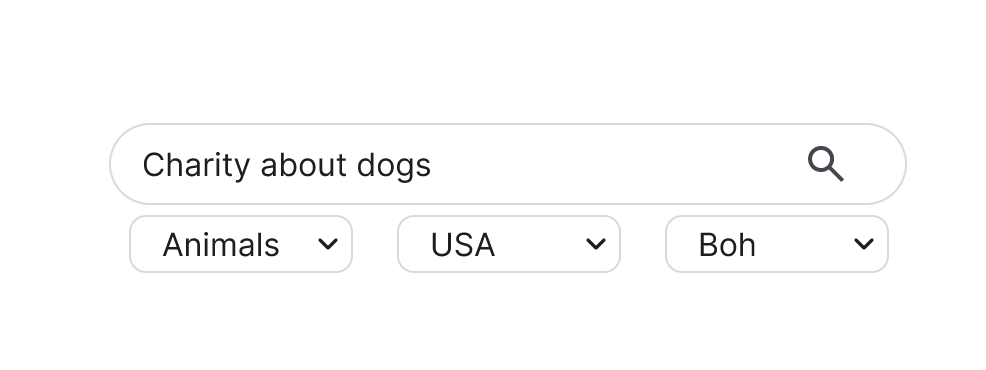
\includegraphics[width=\textwidth]{fig/mockup1.png}
        \caption{Mockup Search Page}
    \end{minipage}\hfill
    \begin{minipage}{0.45\textwidth}
        \centering
        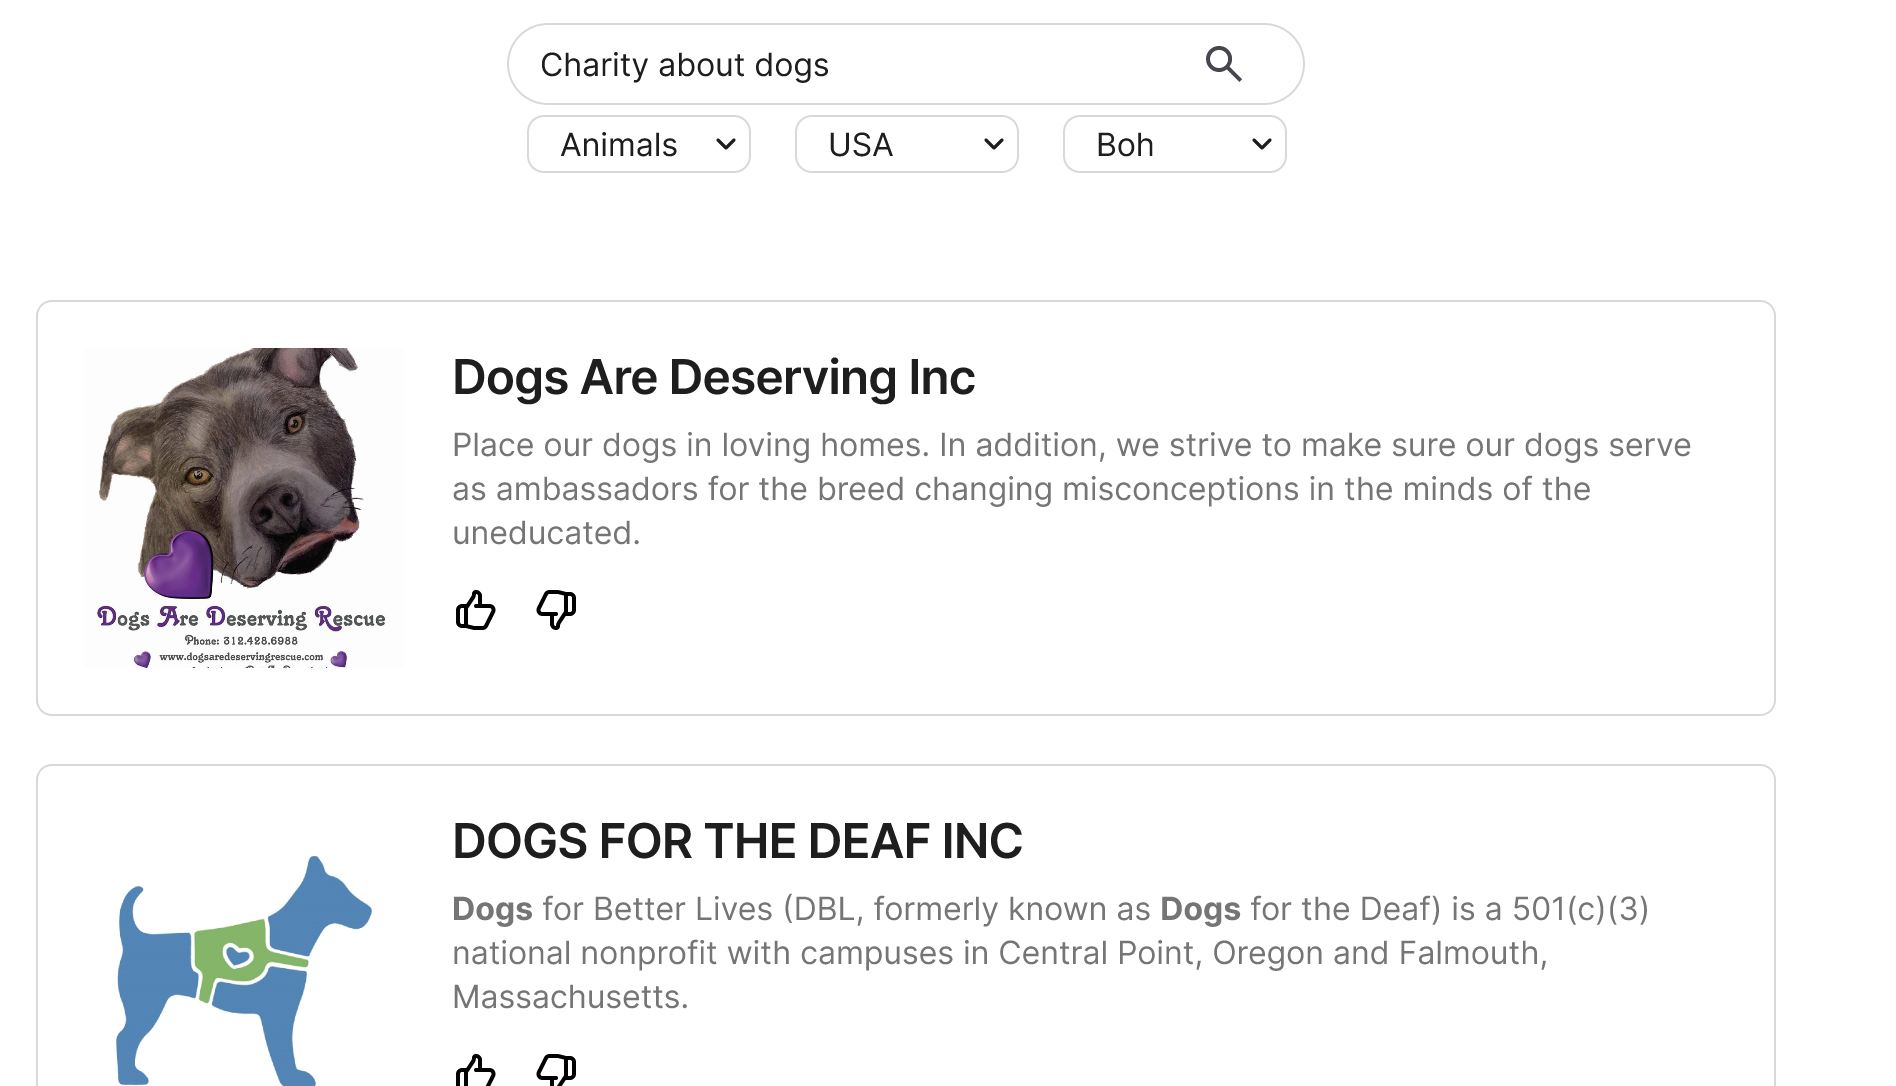
\includegraphics[width=\textwidth]{fig/mockup2.png}
        \caption{Mockup Results Browsing}
    \end{minipage}
\end{figure}

\subsection{Data Collection and Processing}
Costanza is responsible for the data collection and processing. She is in the process of selecting the websites from which information will be retrieved and is currently determining the appropriate scraping techniques and technologies, such as Scrapy and available APIs. She is utilizing a Jupyter Notebook within an Anaconda environment, as recommended during the laboratory sessions.\\
The fields to be stored from the charities are: Name, Logo, Location, Themes, Description, URL of their website, Year of foundation.

\subsection{Backend and Indexing/Retrieval}
Agnese is focusing on the backend and indexing/retrieval part.
We have chosen PyTerrier for indexing and searching the data, and FastAPI to create a simple Python backend that will interface with PyTerrier.
The necessary endpoints for the frontend-backend communication are being defined.
An draft of the main endpoint comprehends parameters for the user query, the filters and the feedback on a result.
\begin{verbatim}
GET /search?q=userQuery&filters=filter1,filter2,filter3&feedback={docId:123,score:1}
\end{verbatim}

\end{document}